\chapter{Code structure}

\section{Introduction}

The original WAQMORF code was developed in FORTRAN.
For \dfastmi we have selected Python because

\begin{itemize}
\item More domain specialists and users are familiar with Python and it's therefore easier for development cycle.
\item Adding a graphical user interface (GUI) is easier in other languages than FORTRAN and by using the same language for kernel and GUI makes the code more consistent and reusable.
\item The algorithm doesn't require large amounts of computations, so a native language isn't needed for adequate performance.
\item The Python environment is available for free contrary to MATLAB which is also widely used in this community.
\item Python supposedly allows for the creation of relatively small redistributable binaries.
\item Python combines well with the open source nature of this software and other developments in the Delft3D / D-HYDRO environment.
\end{itemize}

The software uses a number of Python modules for specific functionality.
Most importantly the code builds on

\begin{itemize}
\item \keyw{netCDF4} for reading and writing netCDF files.
\item \keyw{NumPy} for the numerical computations using arrays.
\item \keyw{PyQt5} for the graphical user interface.
\end{itemize}

The various file formats used and written by \dfastmi are described in the appendix.
The next section describes the subdivision of the code into modules.

\section{Listing of modules}

\dfastmi Python module is subdivided into 8 files:

\begin{itemize}
\item \keyw{\_\_init\_\_.py} module level file containing mainly the version number.
\item \keyw{\_\_main\_\_.py} module level file containing argument parsing and call to \keyw{dfastmi.cmd.run()}.
\item \keyw{cmd.py} containing the main run routine.
\item \keyw{gui.py} for the graphical user interface.
\item \keyw{cli.py} for the interactive command line interface (equivalent to WAQMORF).
\item \keyw{batch.py} for the batch mode.
\item \keyw{io.py} for all file handling: reading of input and configuration files as well as writing of results files.
\item \keyw{kernel.py} for all scientific steps of the algorithm.
\end{itemize}

All files (except for \keyw{\_\_init\_\_.py}) are addressed individually in the following subsections.

\subsection{main function \keyw{cmd.py} and command line interface \keyw{\_\_main\_\_.py}}

The parsing of the command line arguments occurs in \keyw{\_\_main\_\_.py} and the file \keyw{cmd.py} implements the main routine.
The \keyw{\_\_main\_\_} module depends on the \keyw{cmd} module which in turn depends on the \keyw{cli}, \keyw{gui} and \keyw{io} modules.
Depending on the command line arguments \dfastmi will run in one of three modes:

\begin{enumerate}
\item Legacy mode mimicking the existing WAQMORF program (\keyw{cli}).
It uses the same input and output files (report file and SIMONA BOX-files), but uses the new implementation of the algorithm and various configuration files.
\item Batch mode using input file (\keyw{batch}).
It takes the analysis configuration file as input, obtains the relevant data from the old SIMONA files or the new D-Flow FM result files and writes output files (report file and SIMONA BOX-file or netCDF map-file depending on the selected input format).
\item Graphical user interface (\keyw{gui}).
It allows the user to interactively specify the parameters needed for the analysis. The settings can be saved for later batch processing or a batch analysis can be started immediately.
\end{enumerate}

The following command line options are supported

\begin{tabular}{l|l|p{8cm}}
short & long & description \\ \hline
\keyw{-h} & \keyw{-{}-help} & show help text and exit \\
 & \keyw{-{}-rivers} & name of river configuration file (default: \keyw{Dutch\_rivers.ini}) \\
 & \keyw{-{}-language} & language selection: \keyw{NL} or \keyw{UK} (default: \keyw{UK}) \\
 & \keyw{-{}-mode} & run mode \keyw{cli}, \keyw{batch} or \keyw{gui} (default: \keyw{gui})\\
 & \keyw{-{}-config} & name of analysis configuration file (default: \keyw{dfastmi.cfg}) \\
 & \keyw{-{}-reduced\_output} & write reduced SIMONA BOX files (legacy mode only; default: false) \\
\end{tabular}

These files contain one routine each:

\begin{itemize}
\item \keyw{parse\_arguments} parses the command line arguments and returns those values (included in \keyw{\_\_main\_\_.py}).
\item \keyw{run} initializes the language support and starts the appropriate run mode (included in \keyw{cmd.py}).
\end{itemize}

and the main code that triggers the parsing of the command line arguments (via \keyw{parse\_arguments}) and executes \keyw{run} based on those settings.


\subsection{graphical user interface \keyw{gui.py}}

The \keyw{gui.py} module implements the graphical user interface version of \dfastmi.
This module depends on the \keyw{batch}, \keyw{kernel} and \keyw{io} modules.
It can be used to generate and edit the analysis configuration files used for evaluating a single measure.
This run mode is triggered by calling the program using the command line argument \keyw{-{}-mode gui} or by not specifying a \keyw{-{}-mode} argument since this is the default run mode.
It supports both new and old simulation result files.

\begin{figure}
\center
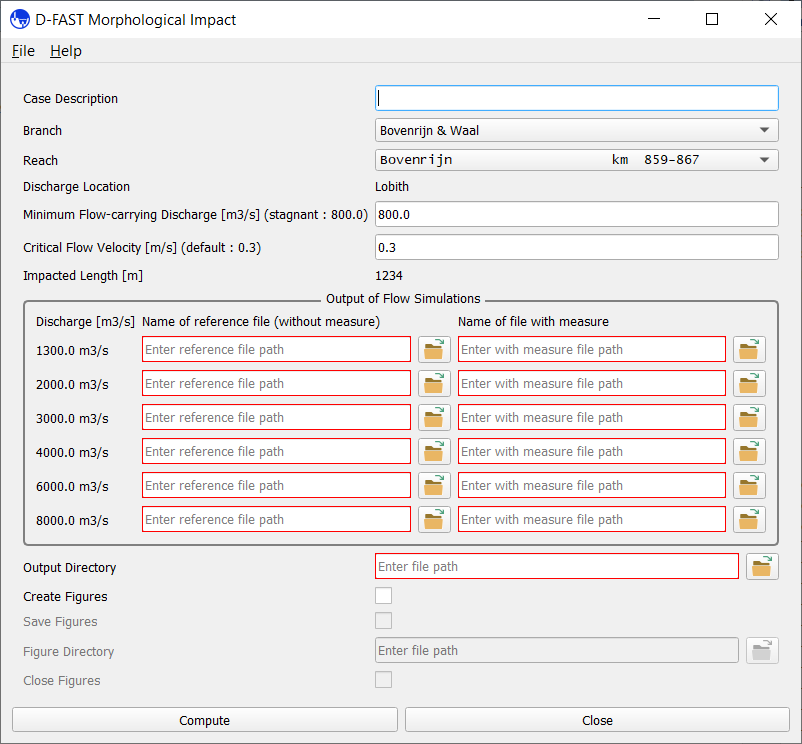
\includegraphics[width=12cm]{figures/main_dialog.png}
\caption{Example of the main dialog}
\end{figure}

This module is subdivided into the following routines:

\begin{itemize}
\item \keyw{gui\_text} obtains a gui text from the global dictionary of dialog texts
\item \keyw{create\_dialog} to create the graphical user interface
\item \keyw{activate\_dialog} to hand over control to the user interface
\item \keyw{updated\_mode} react to a switch between \keyw{WAQUA export} and \keyw{D-Flow FM map} modes
\item \keyw{updated\_branch} react to a change in branch selection
\item \keyw{updated\_reach} react to a change in reach selection
\item \keyw{update\_qvalues} update the discharge values in the dialog and indicate the impacted length
\item \keyw{close\_dialog} support function to close the dialog and end the program
\item \keyw{menu\_load\_configuration} callback function to ask for an analysis configuration file and trigger loading of that file
\item \keyw{load\_configuration} function to actually load an analysis configuration file and update the user interface
\item \keyw{menu\_save\_configuration} callback function to ask for a file name and trigger saving the configuration under that name
\item \keyw{get\_configuration} function to actually extract a configuration from the user interface
\item \keyw{run\_analysis} callback function to run the analysis, generate report and result file (implemented via call to \keyw{batch\_mode})
\item \keyw{menu\_about\_self} and \keyw{menu\_about\_qt} callback functions to show About boxes
\item \keyw{menu\_open\_manual} callback function to open the user manual
\item \keyw{main} main routine creating the user interface, optionally load a configuration, and hand over control to the dialog

\item \keyw{openFileLayout} support function to create a dialog entries of a text field with a browse for file option for all simulation result files options
\item \keyw{selectFile} support function to select a D-Flow FM result file
\item \keyw{showMessage} support function to show a message dialog
\item \keyw{showError} support function to show an error dialog
\end{itemize}


\subsection{interactive command line interface \keyw{cli.py}}

The \keyw{cli.py} module implements the legacy WAQMORF mode of running as an interactive command line program which may be used as batch mode by redirecting standard in; in this mode only result files exported from SIMONA can be used.
This module depends on the \keyw{batch}, \keyw{kernel} and \keyw{io} modules.
This run mode is triggered by calling the program using the command line argument \keyw{-{}-mode cli}.

\begin{itemize}
\item \keyw{interactive\_mode} implements the overall interactive loop
\item \keyw{interactive\_mode\_opening} displays the opening texts of the program
\item \keyw{interactive\_get\_location} implements the interactive selection of the branch/reach location
\item \keyw{interactive\_get\_discharges} implements the interactive selection of the discharges

\item \keyw{write\_report\_nodata} writes the report in case simulation results are not available
\item \keyw{interactive\_check\_discharge} to interactively verify whether simulation results are available for the requested discharges Q1, Q2 and Q3 and if not query for which alternative discharges then
\item \keyw{interactive\_get\_bool}, \keyw{interactive\_get\_int}, \keyw{interactive\_get\_float} and \keyw{interactive\_get\_item} support functions to get boolean, integer, floating point input or branch/reach index from user interaction (legacy mode)
\end{itemize}


\subsection{batch mode \keyw{batch.py}}

The \keyw{batch.py} module executes the analysis in batch mode based on a specified analysis configuration file.
This module depends on the \keyw{kernel} and \keyw{io} modules.
This run mode is triggered by calling the program using the command line argument \keyw{-{}-mode batch}.
It supports both new and old simulation result files.

\begin{itemize}
\item \keyw{batch\_mode} reads the configuration file and triggers the core batch mode analysis
\item \keyw{batch\_mode\_core} carry out the analysis and report the results
\item \keyw{countQ} count the number of discharges for which simulations results need to be provided
\item \keyw{batch\_get\_discharges} extract the discharges to be simulated from the configuration file
\item \keyw{get\_filenames} extract the simulation result file names
\item \keyw{analyse\_and\_report} perform analysis and report results
\item \keyw{analyse\_and\_report\_waqua} perform analysis based on SIMONA result files and report results
\item \keyw{analyse\_and\_report\_dflowfm} perform analysis based on D-Flow Flexible Mesh result files and report results
\item \keyw{get\_values\_waqua1} extract one data column from SIMONA result file
\item \keyw{get\_values\_waqua3} extract three data columns from SIMONA result file
\item \keyw{get\_values\_fm} extract results from a D-Flow Flexible Mesh result file
\item \keyw{write\_report} write the report file
\item \keyw{config\_to\_absolute\_paths} convert all file names in an analysis configuration to absolute paths
\item \keyw{load\_configuration\_file} load a configuration file and adjust file names to absolute paths
\item \keyw{config\_to\_relative\_paths} convert all file names in an analysis configuration to relative paths
\item \keyw{save\_configuration\_file} adjust file names to relative paths and save the configuration file
\item \keyw{stagename} returns the dictionary key for one of the three discharge levels
\end{itemize}


\subsection{general input/output \keyw{io.py}}

The \keyw{io.py} module contains all generic file handling routines for reading configuration files, processing netCDF input and output files, and functions to support legacy input and output formats.
This module does not depend on any other \dfastmi module.

\begin{itemize}
\item \keyw{load\_program\_texts} fills a global dictionary of dialog texts by reading the dialog text configuration file
\item \keyw{log\_text} obtains one text from the global dictionary of dialog texts and writes it to screen or file
\item \keyw{get\_filename} obtains a file name from the global dictionary of dialog texts
\item \keyw{get\_text} obtain one text from the global dictionary of dialog texts

\item \keyw{read\_rivers} reads the rivers configuration file
\item \keyw{collect\_values1} support function for collecting branch/reach data for a parameter with one value, e.g. \keyw{PRHigh}
\item \keyw{collect\_values2} support function for collecting branch/reach data for a parameter with two values, e.g. \keyw{QFit}
\item \keyw{collect\_values4} support function for collecting branch/reach data for a parameter with four values, e.g. \keyw{QLevels}
\item \keyw{write\_config} support function to write a nicely formatted analysis configuration file

\item \keyw{read\_fm\_map} for reading data fields from the D-Flow FM map-file
\item \keyw{get\_mesh\_and\_facedim\_names} for obtaining the name of the 2D mesh and the name of the corresponding face dimension
\item \keyw{copy\_ugrid} for copying UGRID mesh information from the D-Flow FM map-file to the spatial output file
\item \keyw{copy\_var} support function for copying an individual netCDF variable from netCDF file to another
\item \keyw{ugrid\_add} for adding a single cell centred variable to a netCDF file containing UGRID mesh data

\item \keyw{read\_waqua\_xyz} for reading the xyz-files containing data exported from the WAQUA model (legacy function)
\item \keyw{write\_simona\_box} for writing a SIMONA BOX-file (legacy function)

\item \keyw{absolute\_path} converts a relative path into an absolute path given a reference path
\item \keyw{relative\_path} converts an absolute path into a path relative to a given reference path
\item \keyw{get\_progloc} returns the absolute path for the program location
\end{itemize}


\subsection{core algorithm \keyw{kernel.py}}

The \keyw{dfastmi.py} file contains all routines for that perform the mathematical processing steps of the algorithm.
This module does not depend on any other \dfastmi module.

\begin{itemize}
\item \keyw{char\_discharges} for determining the characteristic discharges Q1, Q2 and Q3
\item \keyw{char\_times} for computing the associated time and weight factors
\item \keyw{estimate\_sedimentation\_length} for computing the characteristic length scale of the impact
\item \keyw{dzq\_from\_du\_and\_h} for computing the spatial pattern of dzq based on the change in velocity magnitude and local water depth
\item \keyw{main\_computation} for computing the minimum, mean and maximum impact patterns of the measure on the bed levels after one year
\end{itemize}
